\documentclass[10pt]{beamer}
\usetheme{metropolis}

%own styles
\usepackage{booktabs}
\usepackage[scale=2]{ccicons}
\usepackage{pgfplots}
\usepgfplotslibrary{dateplot}

\usepackage{subfig}
\usepackage{tikz}
\usetikzlibrary{shapes,arrows,positioning}
\usepackage{tikz-uml}
\usepackage[linesnumbered,ruled,vlined]{algorithm2e}
\usepackage{pgfplots}
\usepackage{colortbl}
\usepackage{lscape}
\usepackage{multirow}
\usepackage{amssymb}
\tikzstyle{line} = [draw, -latex']

\usepackage{xspace}
%/own styles

\title{Master Thesis Presentation}
\subtitle{Comparison of Disparity Algorithms for Stereoscopic Videos}
\date{May 25, 2016}
\author{Ben John}
\institute{University of Mannheim, Department of Praktische Informatik IV}

\begin{document}

\maketitle
\setbeamertemplate{frame footer}{Ben John}
\setbeamertemplate{caption}{\raggedright\insertcaption\par}

\begin{frame}{Table of contents}
  \setbeamertemplate{section in toc}[sections numbered]
  \tableofcontents[hideallsubsections]
\end{frame}

\section{Motivation}

\begin{frame}[fragile]{Applications}
  \begin{itemize}
    \item Depth-estimation via camera settings
    \item Kinect (sunlight)
    \item 3DTV (remapping)
  \end{itemize}
\end{frame}

\section{Foundations}

\begin{frame}[fragile]{Epipolar geometry}
  \begin{figure}[h!]
    \centering
    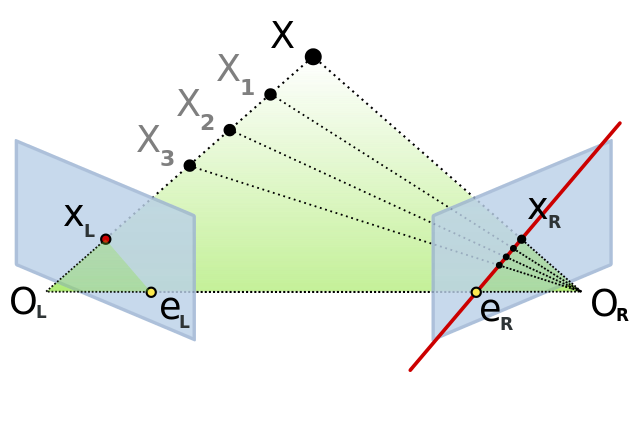
\includegraphics[width=0.6\textwidth]{../paper/src/images/epipolar.png}
    \caption[Epipolar geometry]{Epipolar geometry\protect\footnotemark}
  \end{figure}
  \footnotetext{Source (accessed 02/2016): \url{https://en.wikipedia.org}.}
\end{frame}

\begin{frame}[fragile]{Epipolar geometry}
  \begin{figure}[h!]
    \centering
    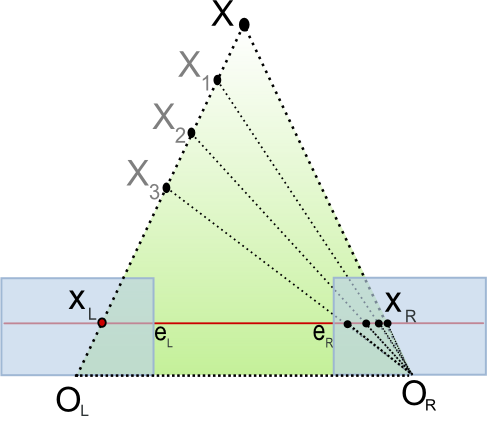
\includegraphics[width=0.5\textwidth]{../paper/src/images/epipolar-rectified.png}
    \caption[Epipolar geometry after image rectification]{Epipolar geometry after image rectification\protect\footnotemark}
  \end{figure}
  \footnotetext{Source (accessed 02/2016): \url{https://en.wikipedia.org}.}
\end{frame}

\begin{frame}[fragile]{Example for stereo image pair}
  \begin{figure}[h!]
  \centering
  \begin{tabular}{ccc}
  \subfloat[left input image]{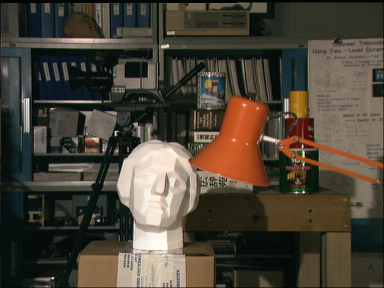
\includegraphics[width=0.3\textwidth]{../paper/src/images/tsukuba-imgL.png}} &
  \subfloat[right input image]{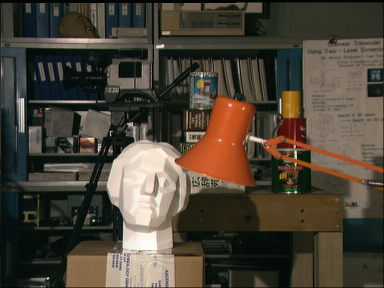
\includegraphics[width=0.3\textwidth]{../paper/src/images/tsukuba-imgR.png}} &
  \subfloat[ground-truth data]{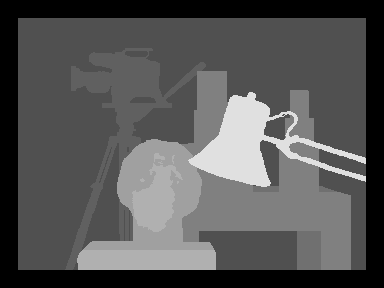
\includegraphics[width=0.3\textwidth]{../paper/src/images/tsukuba-dgt.png}}
  \end{tabular}
  \caption{Tsukuba benchmark stereo image pair of the University of Tsukuba.}
  \end{figure}
\end{frame}

\begin{frame}[fragile]{Classification}
  \begin{itemize}
    \item Global methods
    \begin{itemize}
      \item Dynamic programming
      \item Graph cuts
      \item Belief propagation
    \end{itemize}
    \item Local methods
    \begin{itemize}
      \item Area matching
      \item Feature matching
    \end{itemize}
  \end{itemize}
\end{frame}

\begin{frame}[fragile]{Processing steps}
  \begin{enumerate}
    \item Compute of matching cost
    \item Save values in disparity space image
    \item Aggregate of cost values
    \item Disparity refinement
  \end{enumerate}
\end{frame}

\begin{frame}[fragile]{Step 1: Matching cost}
  \begin{figure}[h!]
    \centering
    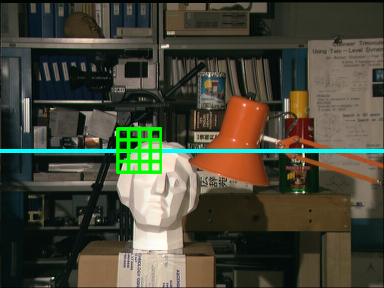
\includegraphics[width=0.5\textwidth]{../paper/src/images/tsukuba-block.png}
    \caption[Block matching along scanlines]{Illustration of block matching along a scanline.}
  \end{figure}
\end{frame}

\begin{frame}[fragile]{Step 2: Disparity space image}
  \begin{figure}[h!]
    \centering
    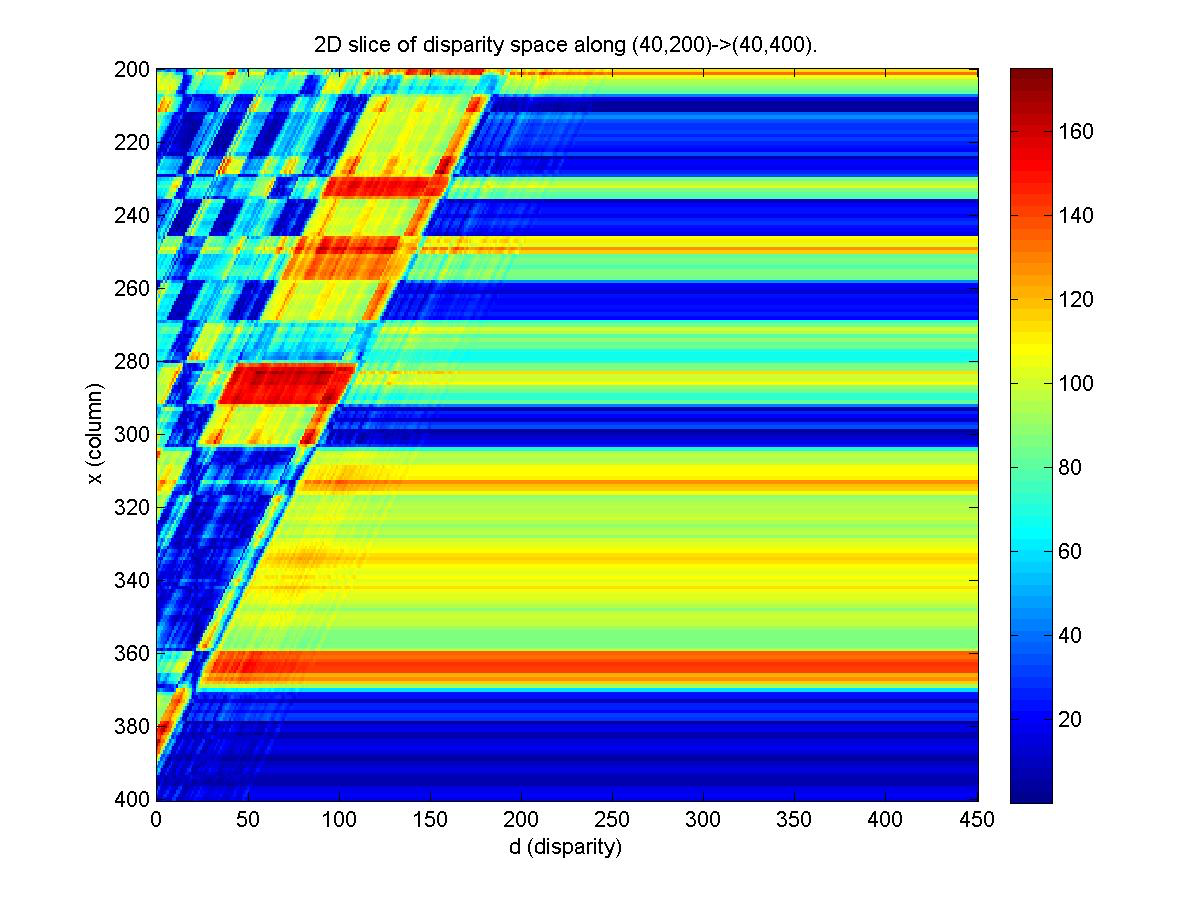
\includegraphics[width=1.0\textwidth]{../paper/src/images/dsi.png}
  \end{figure}
\end{frame}

\section{Implementation}

\tikzstyle{rblock} = [text width=10em, rectangle, draw, fill=blue!20, text centered, rounded corners, minimum height=4em]
\tikzstyle{cloud} = [text width=6em, ellipse, draw, fill=red!15, text centered, rounded corners, minimum height=3.2em]

\begin{frame}[fragile]{Overview}
  \begin{figure}[h!]
    \centering
    \scalebox{0.6}{
    \begin{tikzpicture}[node distance=7em, auto]
      %input
      \node [cloud] (right) {right image};
      \node [cloud, right of=right, node distance=10em] (left) {left image};
      \node [cloud, right of=left, node distance=10em] (disp) {ground-truth};
  
      %computation
      \node [rblock, below of=right, xshift=2em] (exec) {(1) Algorithm executor};
      \node [rblock, below of=disp, xshift=-2em] (mask-creator) {(2) Mask creator};
      
      %diminisher
      \node [rblock, above of=exec, yshift=7em] (dim) {(4) Image diminisher};
  
      %output
      \node [cloud, below of=exec] (map) {disparity map};
      \node [cloud, below of=mask-creator] (masks) {masks};
  
      %evaluation
      \node [rblock, below of=left, yshift=-14em] (evaluation) {(3) Disparity evaluator};
  
      %final result
      \node [cloud, below of=evaluation, xshift=-5em] (csv) {CSV file};
      \node [cloud, below of=evaluation, xshift=5em] (heatmaps) {heatmaps};
  
      %lines
      \path [line] (dim) -- (right);
      \path [line] (dim) -- (left);
      
      \path [line] (right) -- (exec);
      \path [line] (left) -- (exec);
      \path [line] (left) -- (mask-creator);
      \path [line] (disp) -- (mask-creator);
  
      \path [line] (exec) -- (map);
      \path [line] (mask-creator) -- (masks);
  
      \path [line] (map) -- (evaluation);
      \path [line] (masks) -- (evaluation);
  
      \path [line] (evaluation) -- (csv);
      \path [line] (evaluation) -- (heatmaps);
    \end{tikzpicture}
    }
    \caption[Composition and processing pipeline of the implementation]{Composition and processing pipeline of the implementation.}
  \end{figure}
\end{frame}

\begin{frame}[fragile]{Spatiotemporal stereo matcher (1)}
  \scalebox{0.86}{
    \begin{algorithm}[H]
    \DontPrintSemicolon
    \KwIn{$\{I_L\}$, $\{I_R\}$, $d_{max}$, $wSize$}
    \KwOut{$C$}
    $step \gets (wSize - 1) / 2$\;
    $C \gets \textsc{CreateMatrix}(\textsc{Cols}(I_L),\textsc{Rows}(I_L),\textsc{Images}(I_L),d_{max})$\;
    \For{$t \gets 0$ \textbf{to} $\textsc{Images}(I_L)$} {
      $leftImage \gets I_L(t)$\;
      $rightImage \gets I_L(t)$\;
      \For{$y \gets 0 + step$ \textbf{to} $\textsc{Rows}(I_L(0)) - step$} {
        \For{$x \gets 0 + step$ \textbf{to} $\textsc{Cols}(I_L(0)) - step - d_{max}$} {
          \For{$d \gets 0$ \textbf{to} $d_{max}$} {
            $rect_{L} \gets \textsc{Rect}\{x - step, y - step, wSize, wSize\}$\;
            $rect_{R} \gets \textsc{Rect}\{x + d - step, y - step, wSize, wSize\}$\;
            $window_{L} \gets leftImage(rect_{L})$\;
            $window_{R} \gets rightImage(rect_{R})$\;
            $C(x,y,t,d) \gets \textsc{MatchingCost}(window_{L}, window_{R})$\;
          }
        }
      }
    }
    \Return{$C$}\;
    \caption{\textsc{CreateDisparitySpaceImage}}
    \end{algorithm}

  }
\end{frame}

\begin{frame}[fragile]{Spatiotemporal stereo matcher (2)}
  \scalebox{1.0}{
    \begin{algorithm}[H]
    \DontPrintSemicolon
    \KwIn{$C$, $t$}
    \KwOut{$DisparityMap$}
    $DisparityMap \gets \textsc{CreateMatrix}(\textsc{Cols}(C),\textsc{Rows}(C))$\;
    \For{$t \gets 0$ \textbf{to} $\textsc{Frames}(C)$} {
      \For{$y \gets 0$ \textbf{to} $\textsc{Rows}(C)$} {
        \For{$x \gets 0$ \textbf{to} $\textsc{Cols}(C)$} {
          $Cost \gets \frac{1}{4} C(x,y,f_{t-1}) + \frac{2}{4} C(x,y,f_{t})+ \frac{1}{4} C(x,y,f_{t+1})$\;
          $DisparityMap(x,y) \gets \textsc{BestMatch}(Cost)$\;
        }
      }
    }
    \Return{$DisparityMap$}\;
    \caption{\textsc{GetDisparityMap}}
    \end{algorithm}
  }
\end{frame}

\begin{frame}[fragile]{Masking modes}
  \begin{columns}[onlytextwidth]
    \column{0.5\textwidth}
      \begin{itemize}
        \item Non-occluded mask
        \item Depth-discontinuity mask
        \item Textureless mask
        \item Saliency mask
      \end{itemize}
    \column{0.5\textwidth}
    \only<1>{
      \begin{figure}
      \centering
      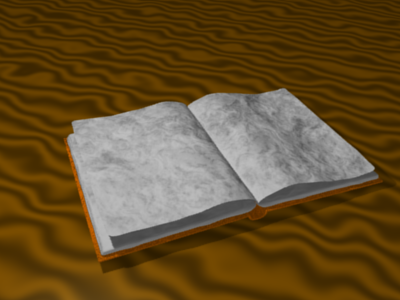
\includegraphics[width=1.0\textwidth]{images/book-img.png}
      \caption{Frame of book sequence}
      \end{figure}
    }
    \only<2>{
      \begin{figure}
      \centering
      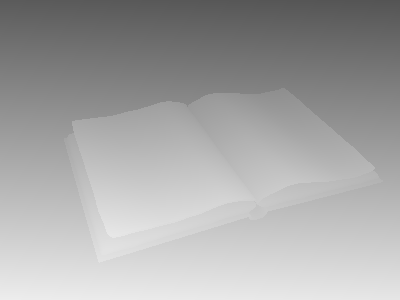
\includegraphics[width=1.0\textwidth]{images/book-truth.png}
      \caption{Ground-truth disparity map}
      \end{figure}
    }
    \only<3>{
      \begin{figure}
      \centering
      {%
      \setlength{\fboxsep}{0pt}%
      \setlength{\fboxrule}{1pt}%
      \fbox{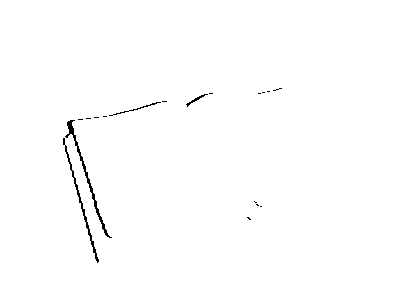
\includegraphics[width=1.0\textwidth]{images/book-mask-noc.png}
      }%
      }%
      \caption{Non-occluded mask}
      \end{figure}
    }
    \only<4>{
      \begin{figure}
      \centering
      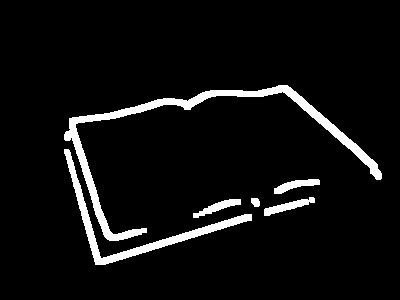
\includegraphics[width=1.0\textwidth]{images/book-mask-dd.png}
      \caption{Depth-discontinuity at object borders}
      \end{figure}
    }
    \only<5>{
      \begin{figure}
      \centering
      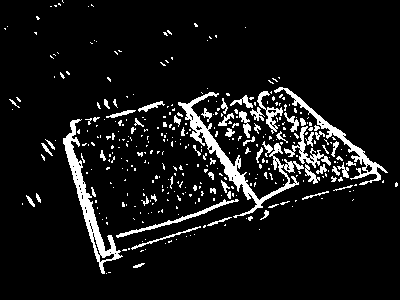
\includegraphics[width=1.0\textwidth]{images/book-mask-tex.png}
      \caption{Textureless regions}
      \end{figure}
    }
    \only<6>{
      \begin{figure}
      \centering
      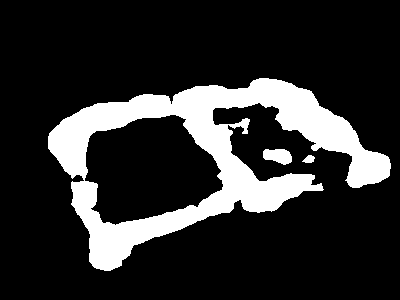
\includegraphics[width=1.0\textwidth]{images/book-mask-sal.png}
      \caption{Salient pixels}
      \end{figure}
    }
  \end{columns}
\end{frame}

\begin{frame}[fragile]{Web viewer}
  \begin{columns}[onlytextwidth]
    \column{0.5\textwidth}
    \begin{itemize}
      \item Visualization of evaluation engine
      \item Written in Node.js
      \item Displaying statistical information
    \end{itemize}
    \column{0.5\textwidth}
      \begin{figure}
      \centering
      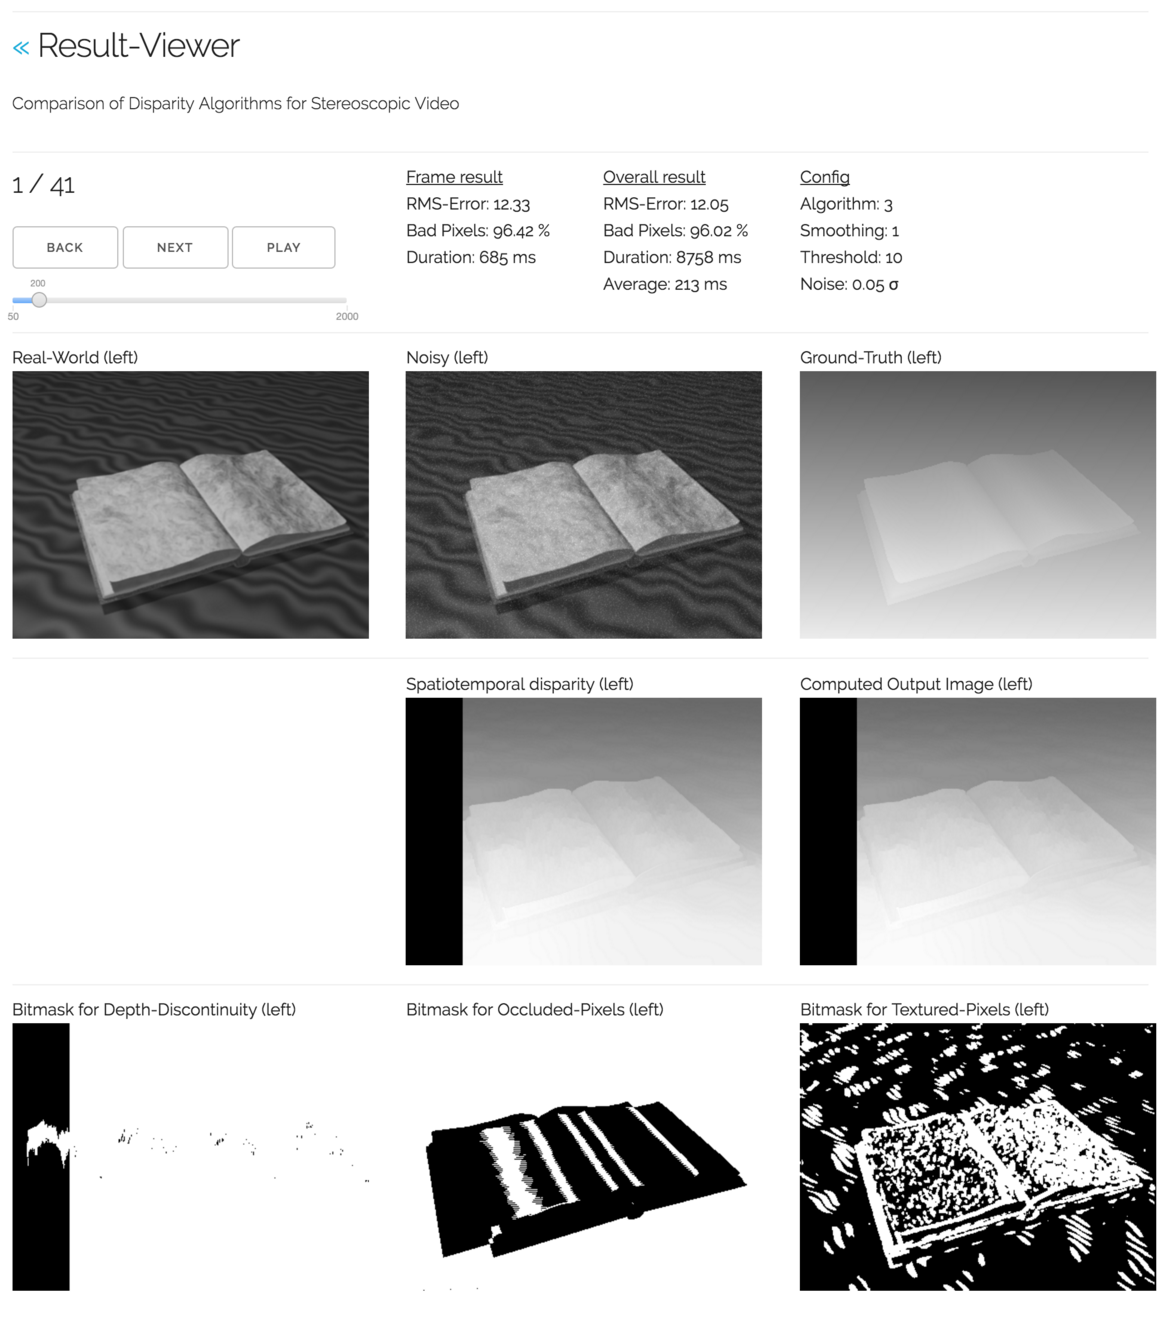
\includegraphics[width=1.0\textwidth]{../paper/src/images/result-viewer-detail.png}
      \caption{Detail view}
      \end{figure}
  \end{columns}
\end{frame}

\plain{Demo}

\section{Evaluation}

\begin{frame}[fragile]{Overview}
  \begin{block}{Analyzed algorithms}
    \begin{itemize}
      \item OpenCV implementations
      \begin{itemize}
        \item (1) Semi-global stereo matcher
        \item (2) Block matcher
        \item (10) Simple block matcher
      \end{itemize}
      \item (3) Efficient large scale stereo matcher (ELAS)
      \item Middlebury MRF library
      \begin{itemize}
        \item (4) Iterated conditional modes (ICM)
        \item (5-6) Graph cuts (swap and extension)
        \item (7-9) Various belief propagations implementations
      \end{itemize}
      \item Own stereo matcher implementation
      \begin{itemize}
        \item (11) Simple block-matcher
        \item (12-13) Simple spatiotemporal consistent block-matcher
      \end{itemize}
    \end{itemize}
  \end{block}
\end{frame}

\begin{frame}[fragile]{Datasets (1)}
  \begin{block}{Cambridge}
    \begin{itemize}
      \item 5 sequences
      \item at 500 x 400 resolution
    \end{itemize}
    \begin{figure}
    \centering
    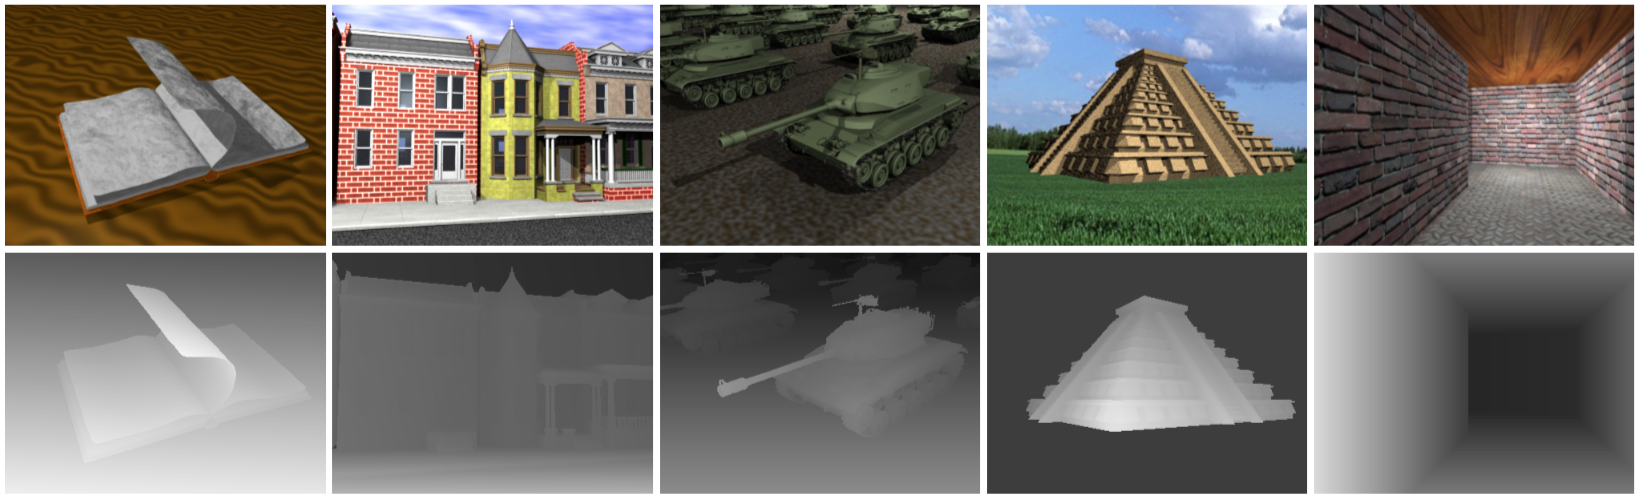
\includegraphics[width=1.0\textwidth]{../paper/src/images/dbcgrid-dataset.png}
    \caption{Overview of sequences}
    \end{figure}
  \end{block}
\end{frame}

\begin{frame}[fragile]{Datasets (2)}
  \begin{block}{SVDDD}
    \begin{itemize}
      \item 2 sequences
      \item at 1920 x 1080 resolution
    \end{itemize}
    \begin{figure}
    \centering
    \begin{tabular}{cc}
    \subfloat[02 rabbit scene]{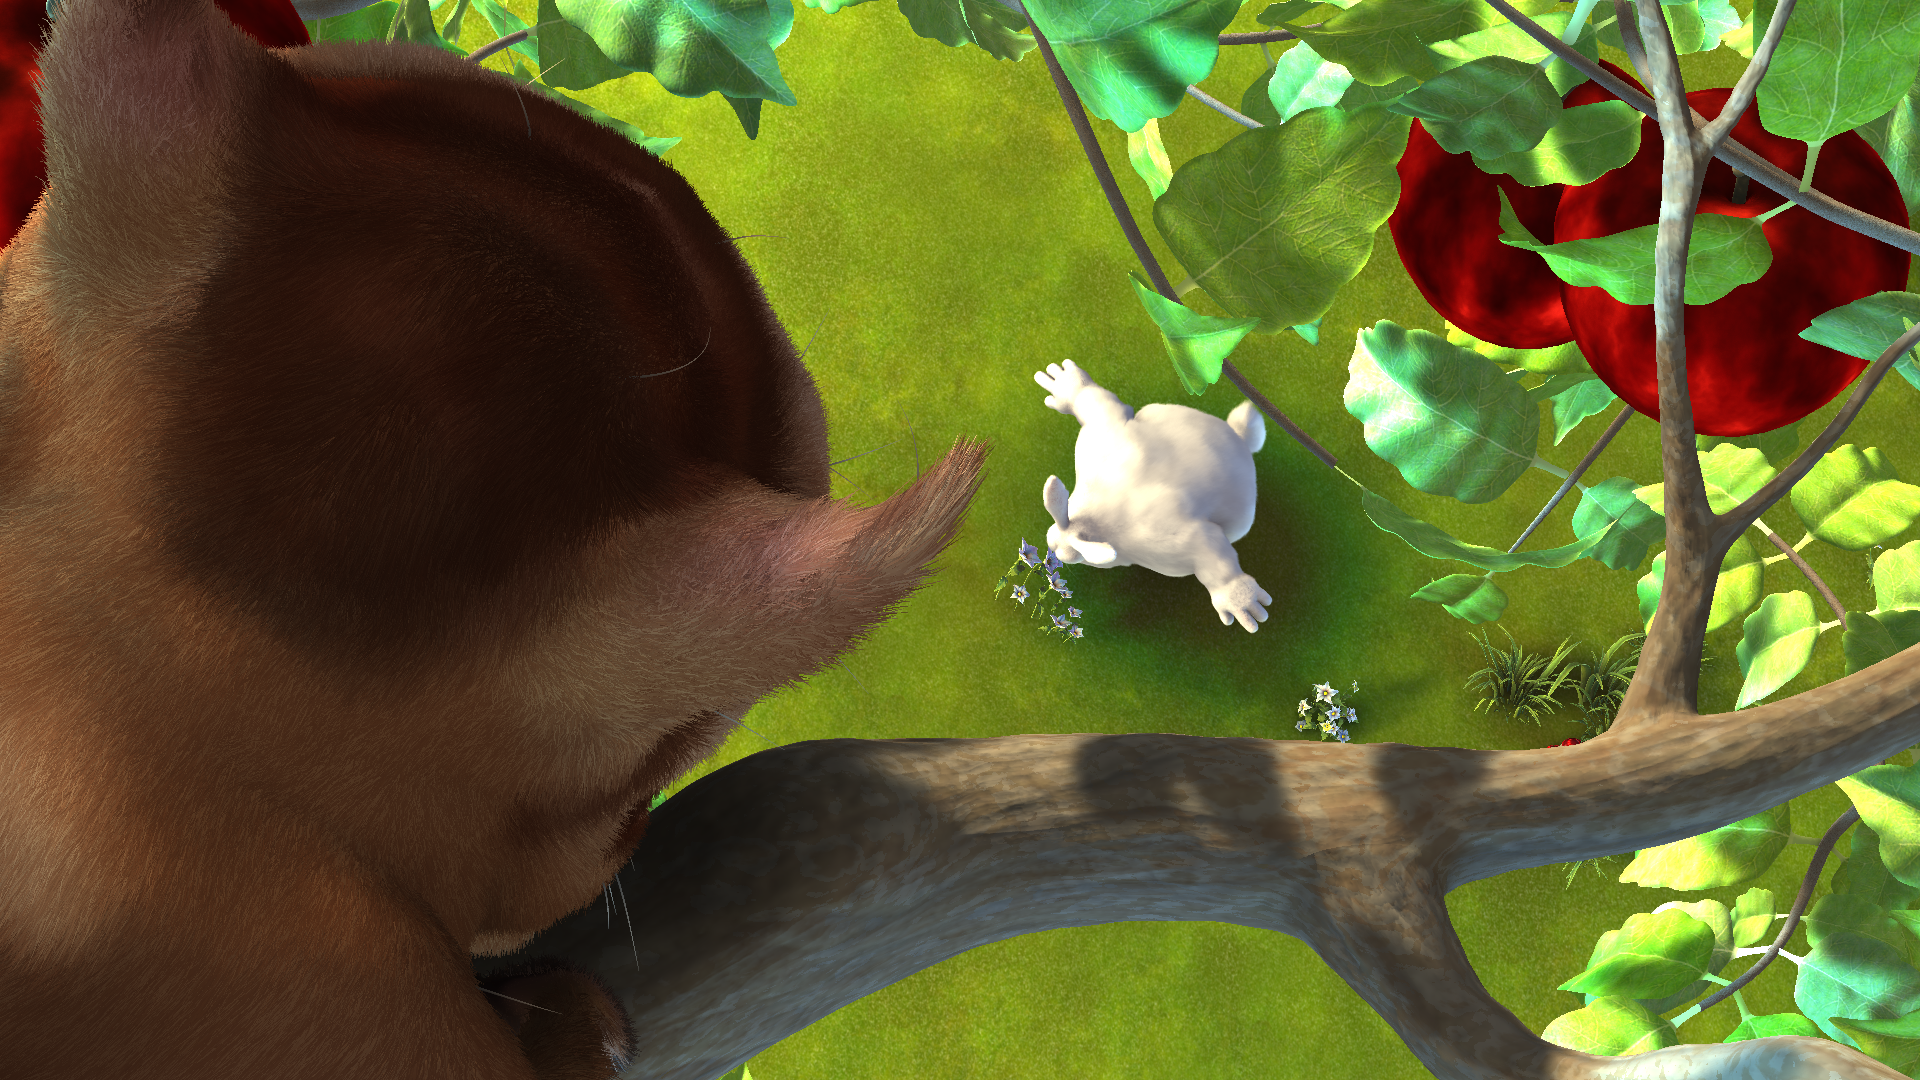
\includegraphics[width=0.45\textwidth]{images/02-rabbit.png}} &
    \subfloat[03 apple scene]{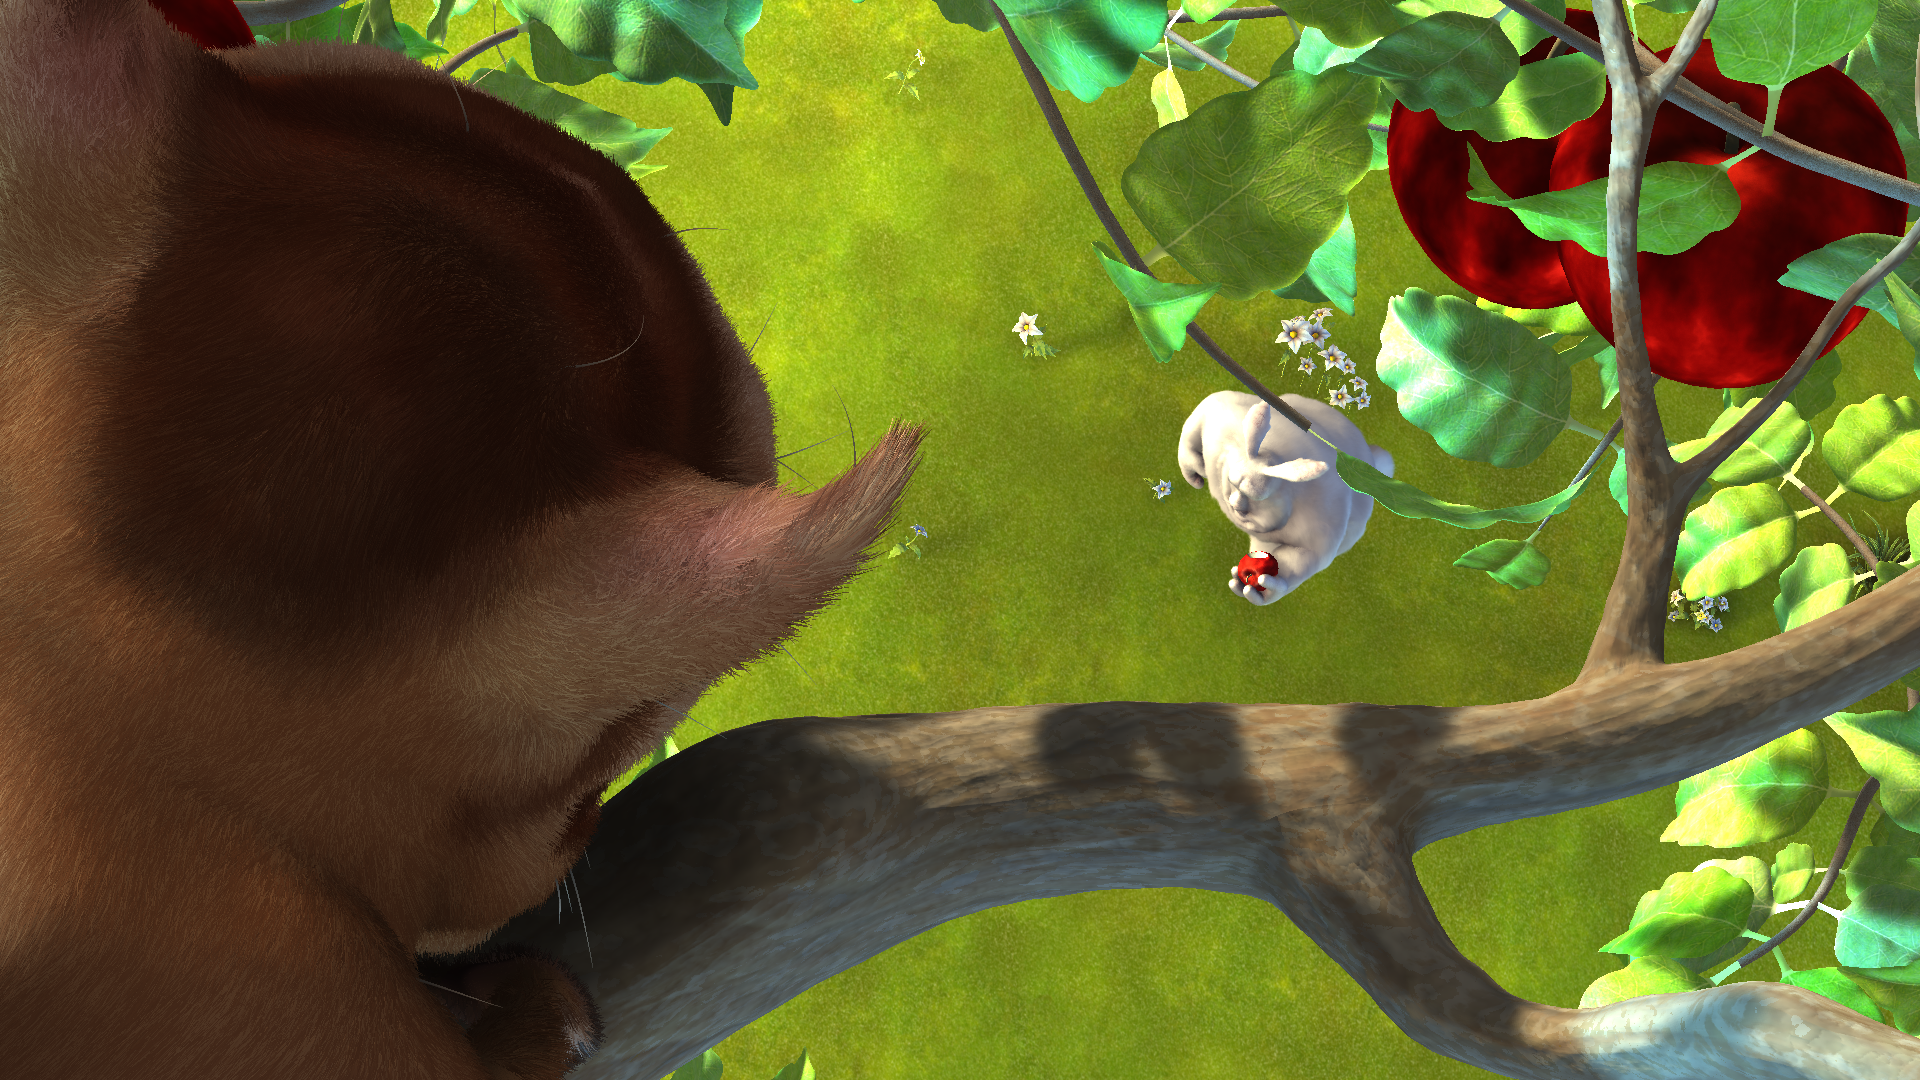
\includegraphics[width=0.45\textwidth]{images/03-apple.png}} \\
    \end{tabular}
    \caption{Overview of sequences}
    \end{figure}
  \end{block}
\end{frame}

\begin{frame}[fragile]{Metrics}
  \begin{itemize}
    \item \begin{block}{Percentage of bad matching pixels}
      $\frac{1}{n} \sum_{x,y=0}^{}(|d_a(x,y) - d_e(x,y)| > \delta_t)$
    \end{block}
    \item \begin{block}{RMS-Error}
      $\sqrt{\frac{1}{n} \sum_{x,y=0}^{}(|d_a(x,y) - d_e(x,y)|)^2}$
    \end{block}
  \end{itemize}
\end{frame}

\begin{frame}[fragile]{Results (1) - Own stereo matcher}
  \begin{table}
  \centering
  \scalebox{1.0}{
  \begin{tabular}{l|rrrr}
    & 10 CVSM & 11 SNSM & 12 SNTU & 13 SNTW \\ \hline
  S1 - book & \cellcolor{red!50}32.61\% & \cellcolor{green!50}8.72\% & 10.07\% & 9.65\% \\
  S2 - street & \cellcolor{red!50}25.64\% & 11.79\% & \cellcolor{green!50}8.76\% & 8.90\% \\
  S3 - tanks & \cellcolor{red!50}13.26\% & \cellcolor{green!50}6.08\% & 8.71\% & 7.29\% \\
  S4 - temple & \cellcolor{red!50}38.96\% & 12.98\% & \cellcolor{green!50}11.15\% & 11.26\% \\
  S5 - tunnel & \cellcolor{red!50}8.60\% & \cellcolor{green!50}0.93\% & 4.54\% & 2.15\% \\ \hline
  $\varnothing$ & \cellcolor{red!50}23,81\% & 8,10\% & 8,66\% & \cellcolor{green!50}7,85\% 
  \end{tabular}
  }
  \caption{Result table for comparison of own implementation with Cambridge dataset}
  \end{table}
\end{frame}

\begin{frame}[fragile]{Results (2) - Outliers}
  \begin{figure}[h!]
  \centering
  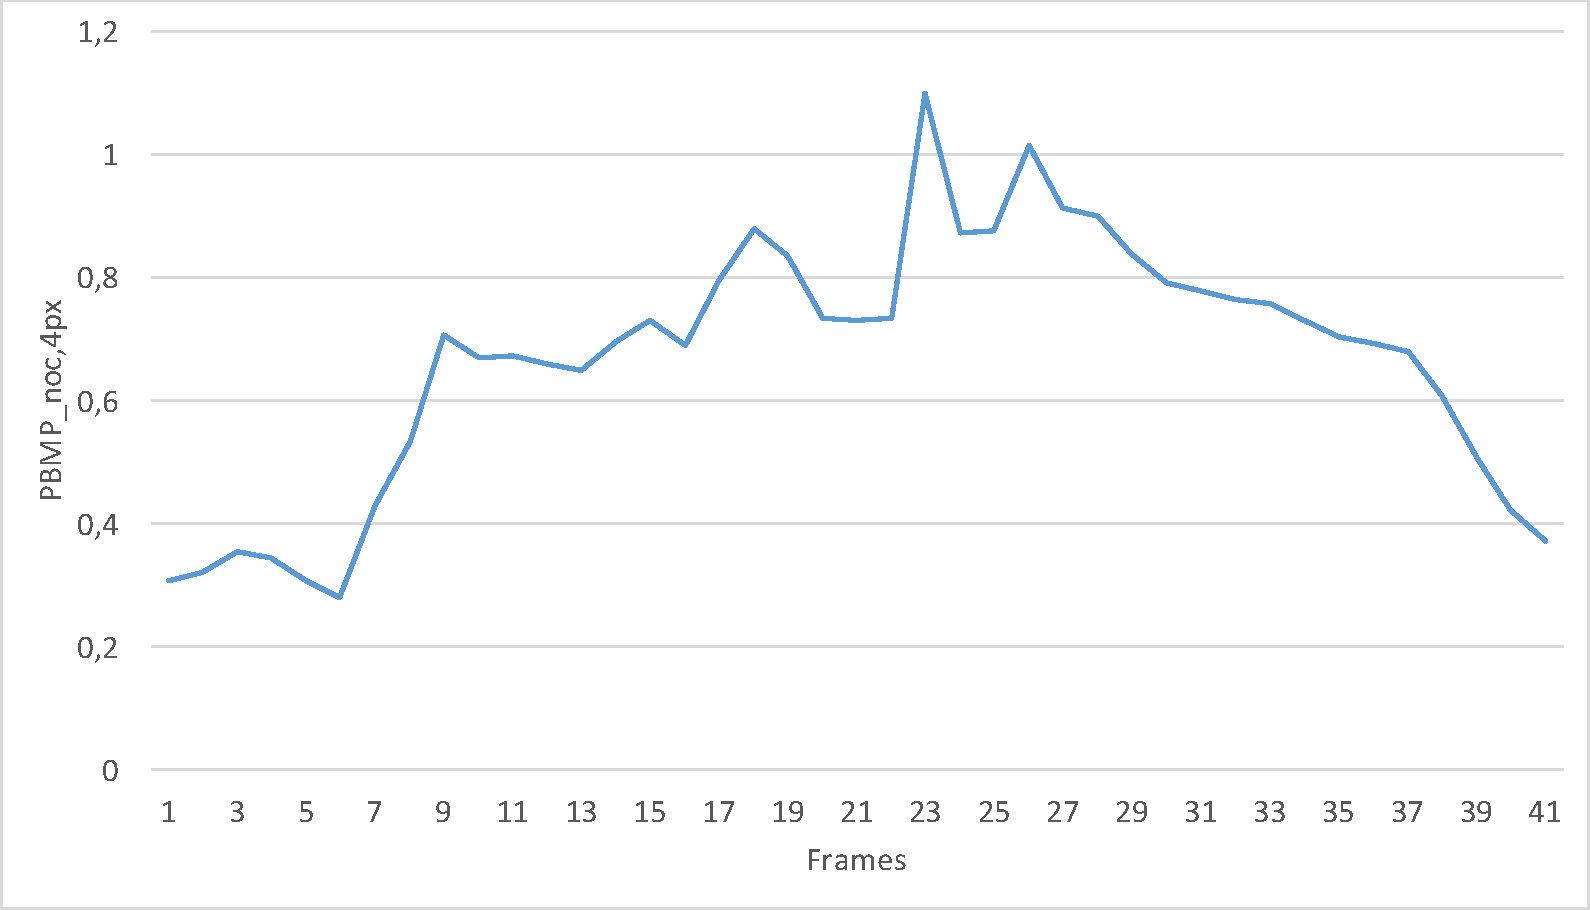
\includegraphics[width=1.0\textwidth]{../paper/src/images/evaluation/plots/01-book-general-outliers.pdf}
  \caption{Chart of general outliers in the book sequence with ELAS algorithm.}
  \end{figure}
\end{frame}

\begin{frame}[fragile]{Results (3) - Outliers example}
  \begin{figure}[h!]
  \centering
  \begin{tabular}{ccc}
  \subfloat[Frame 1]{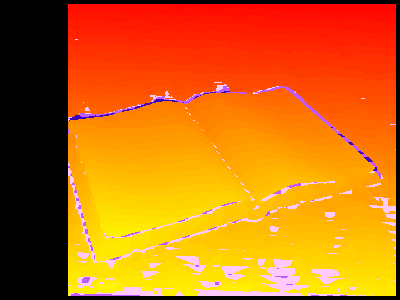
\includegraphics[width=0.3\textwidth]{../paper/src/images/evaluation/outliers/image0001.png}} &
  \subfloat[Frame 23]{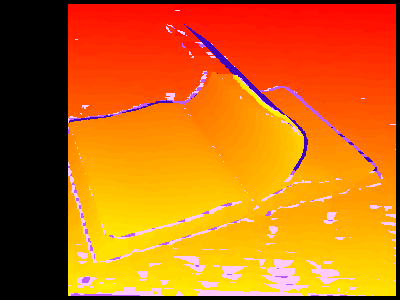
\includegraphics[width=0.3\textwidth]{../paper/src/images/evaluation/outliers/image0023.png}} &
  \subfloat[Frame 26]{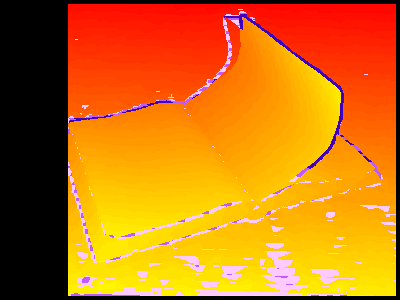
\includegraphics[width=0.3\textwidth]{../paper/src/images/evaluation/outliers/image0026.png}} \\
  \end{tabular}
  \caption{Examples for general outliers in the book sequence. The disparity maps are computed with the (3) ELAS algorithm.}
  \end{figure}
\end{frame}

\begin{frame}[fragile]{Results (4) - Video compression}
  \begin{figure}[h!]
  \centering
  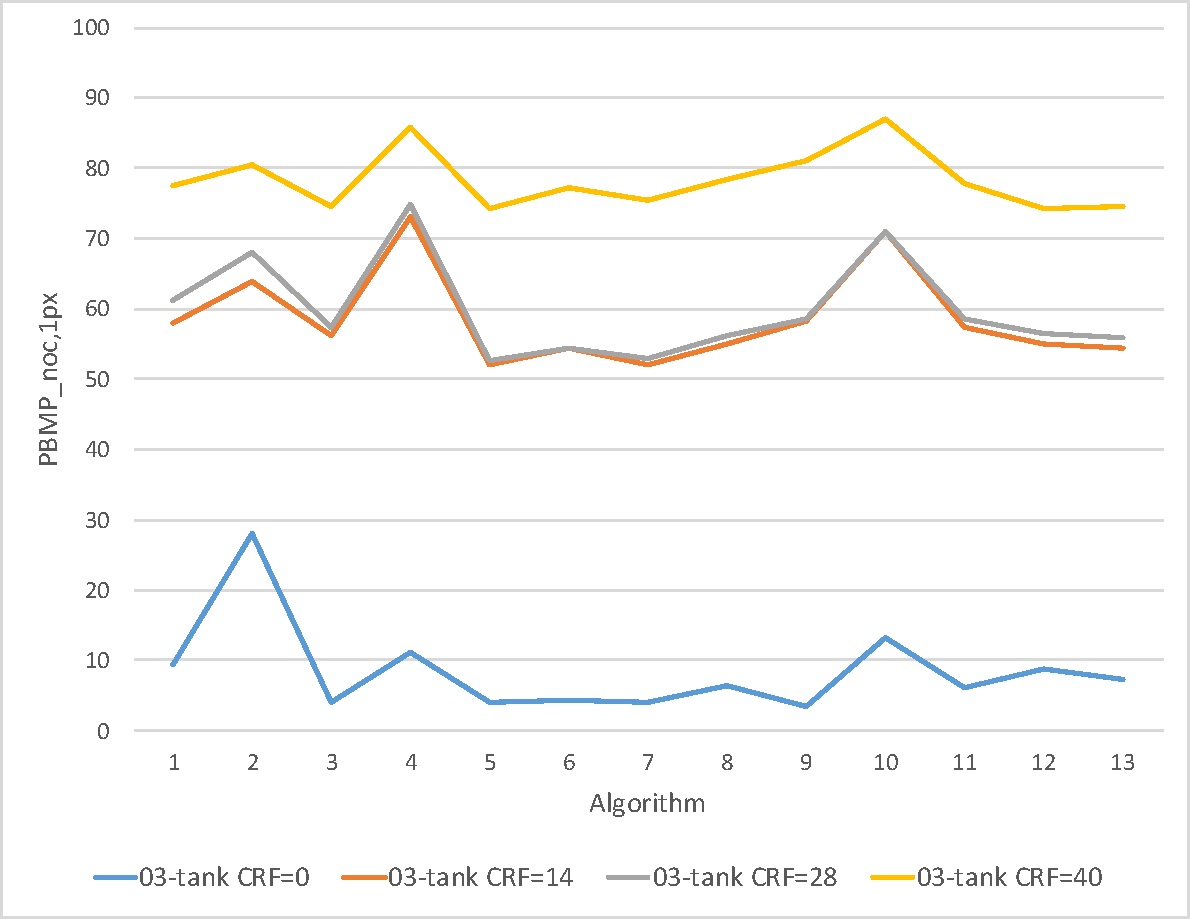
\includegraphics[width=0.8\textwidth]{../paper/src/images/evaluation/plots/03-tank-pbmp-noc-1-vc.pdf}
  \caption[Chart of the impact of video compression]{Chart of the impact of different CRF values for H.265 video compression on the result of disparity algorithms focusing on PBMP$_{noc,1px}$.}
  \label{fig:eval-plots-pbmp-noc1-vc}
  \end{figure}
\end{frame}

\begin{frame}[fragile]{Results (5) - Video compression examples}
  \begin{figure}[h!]
  \centering
  \begin{tabular}{ccc}
  \subfloat[(3) ELAS outliers]{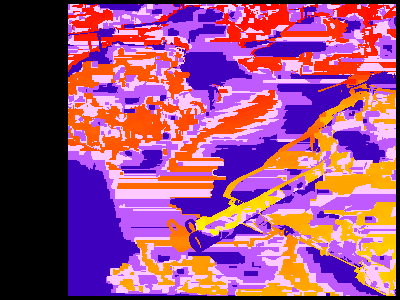
\includegraphics[width=0.3\textwidth]{../paper/src/images/evaluation/outliers-vc/image0023-heatmap-outliers-3.png}} &
  \subfloat[(5) MRF GC Swap outliers]{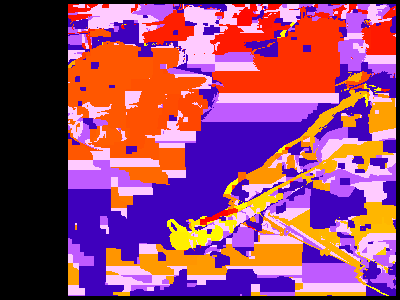
\includegraphics[width=0.3\textwidth]{../paper/src/images/evaluation/outliers-vc/image0023-heatmap-outliers-5.png}} &
  \subfloat[(13) SNSM STW]{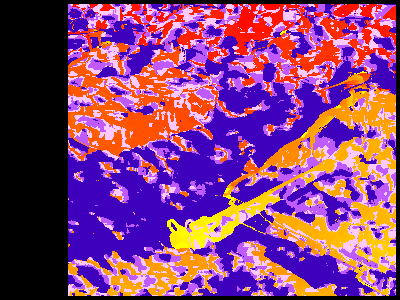
\includegraphics[width=0.3\textwidth]{../paper/src/images/evaluation/outliers-vc/image0023-heatmap-outliers-13.png}} \\
  \end{tabular}
  \caption[Example of computed disparity maps with video compression]{Example of computed disparity maps with video compression. CRF is set to $40$. Frame 23 of the tanks scene.}
  \label{fig:eval:vc:eg2}
  \end{figure}
\end{frame}

\begin{frame}[fragile]{Results (6) - Runtime}
  \begin{figure}[h!]
  \centering
  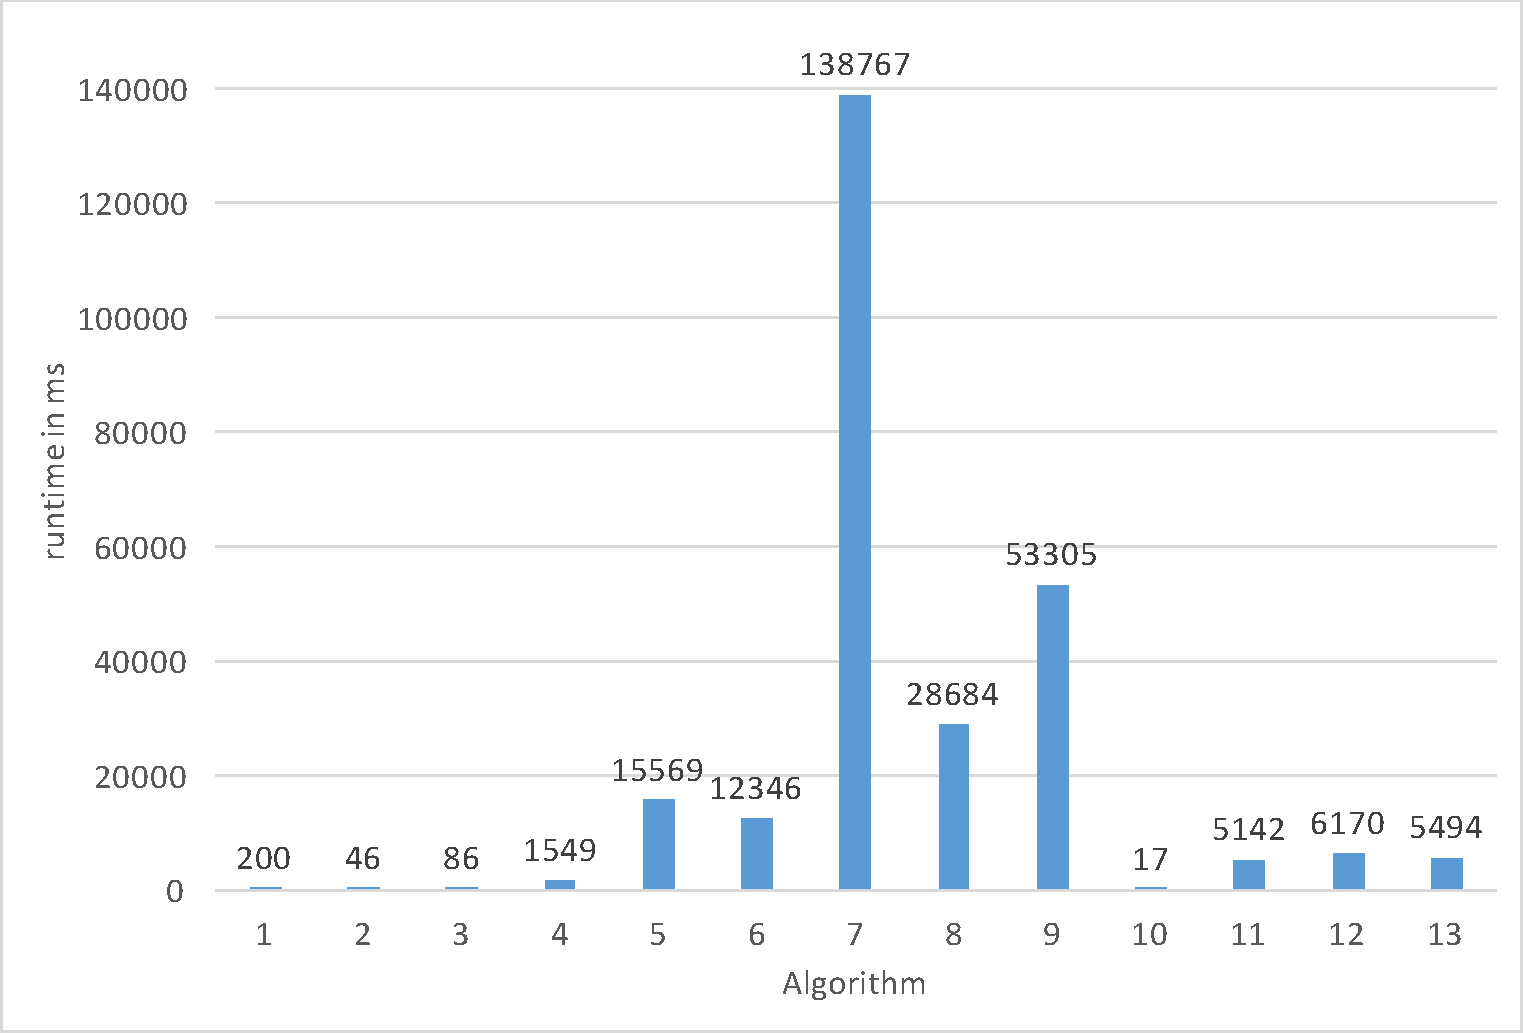
\includegraphics[width=0.8\textwidth]{../paper/src/images/evaluation/plots/runtime.pdf}
  \caption{Comparison of the runtime of different disparity algorithms.}
  \end{figure}
\end{frame}

\begin{frame}[fragile]{Results (7) - SVDDD}
  \begin{figure}[h!]
  \centering
  \begin{tabular}{ccc}
  \subfloat[Negative disparity]{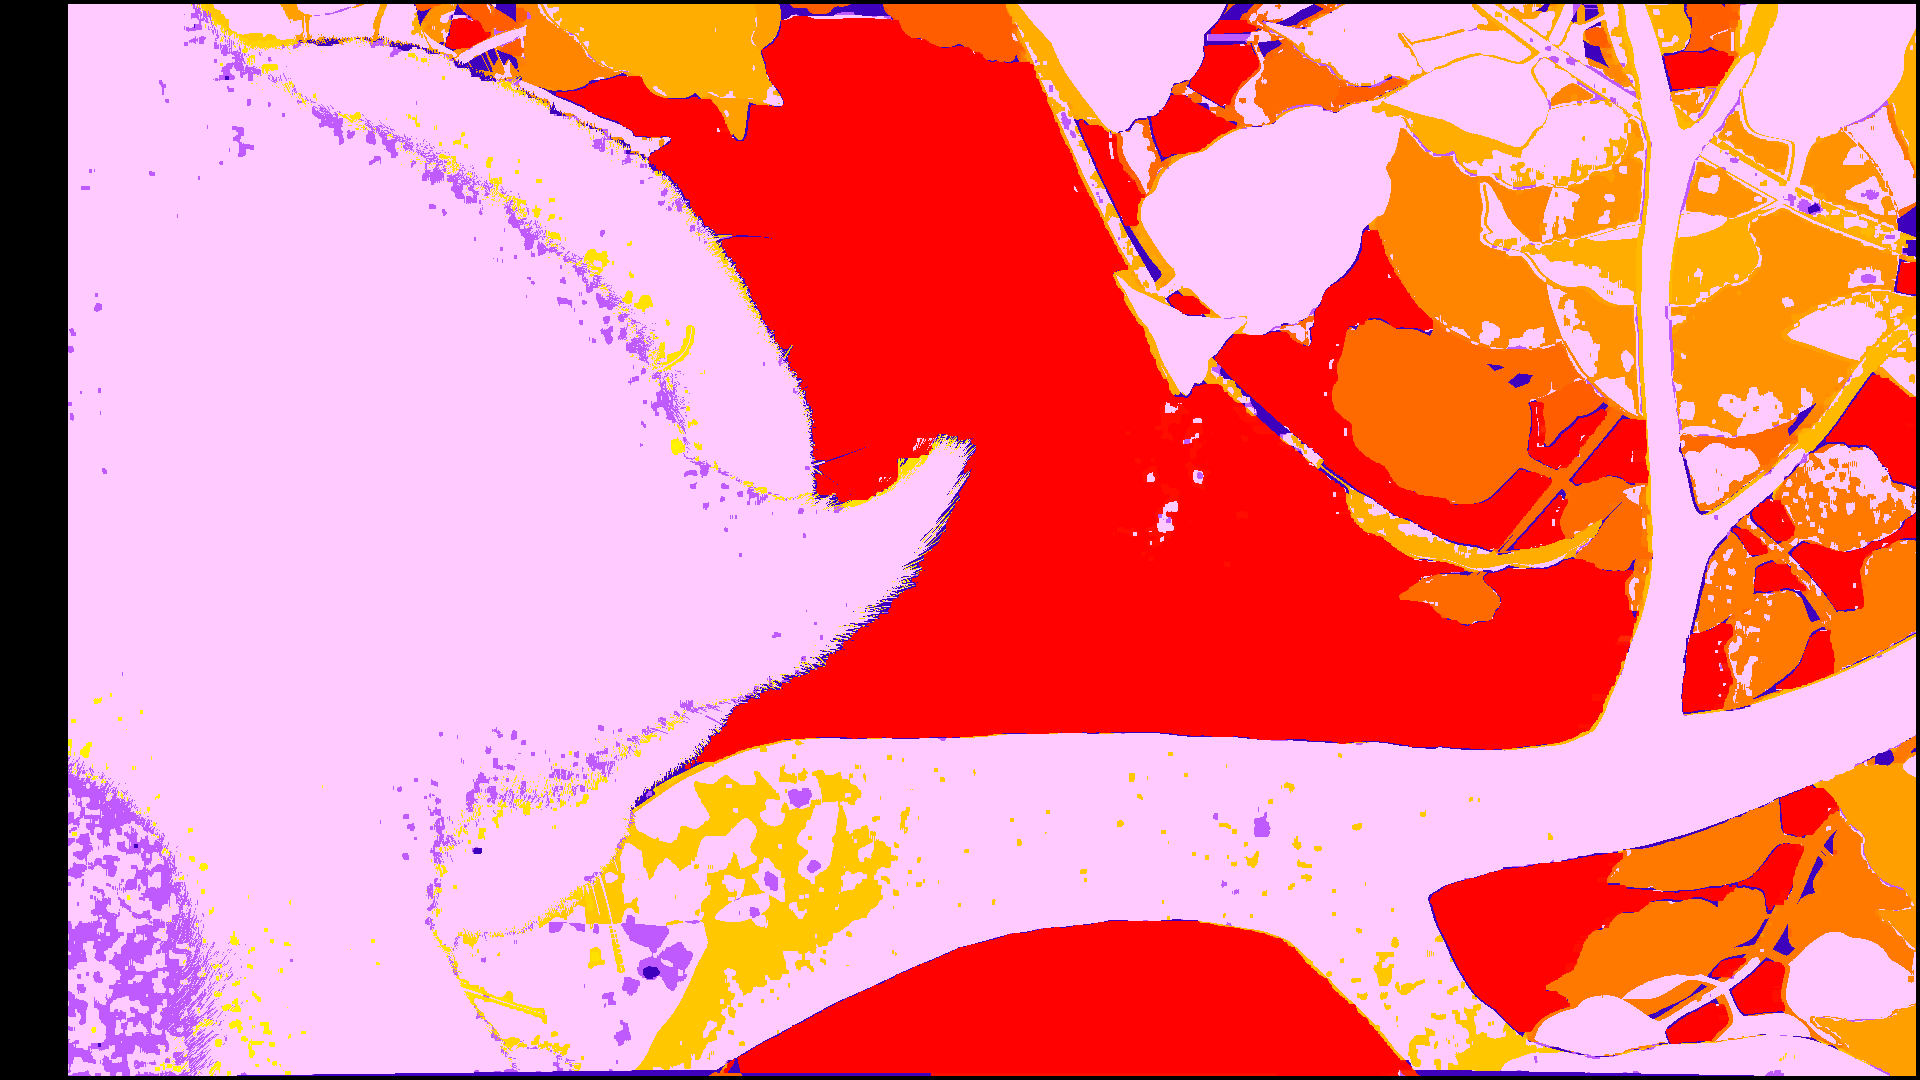
\includegraphics[width=0.48\textwidth]{../paper/src/images/evaluation/02-rabbit-neg-elas.png}} &
  \subfloat[Only positive disparity]{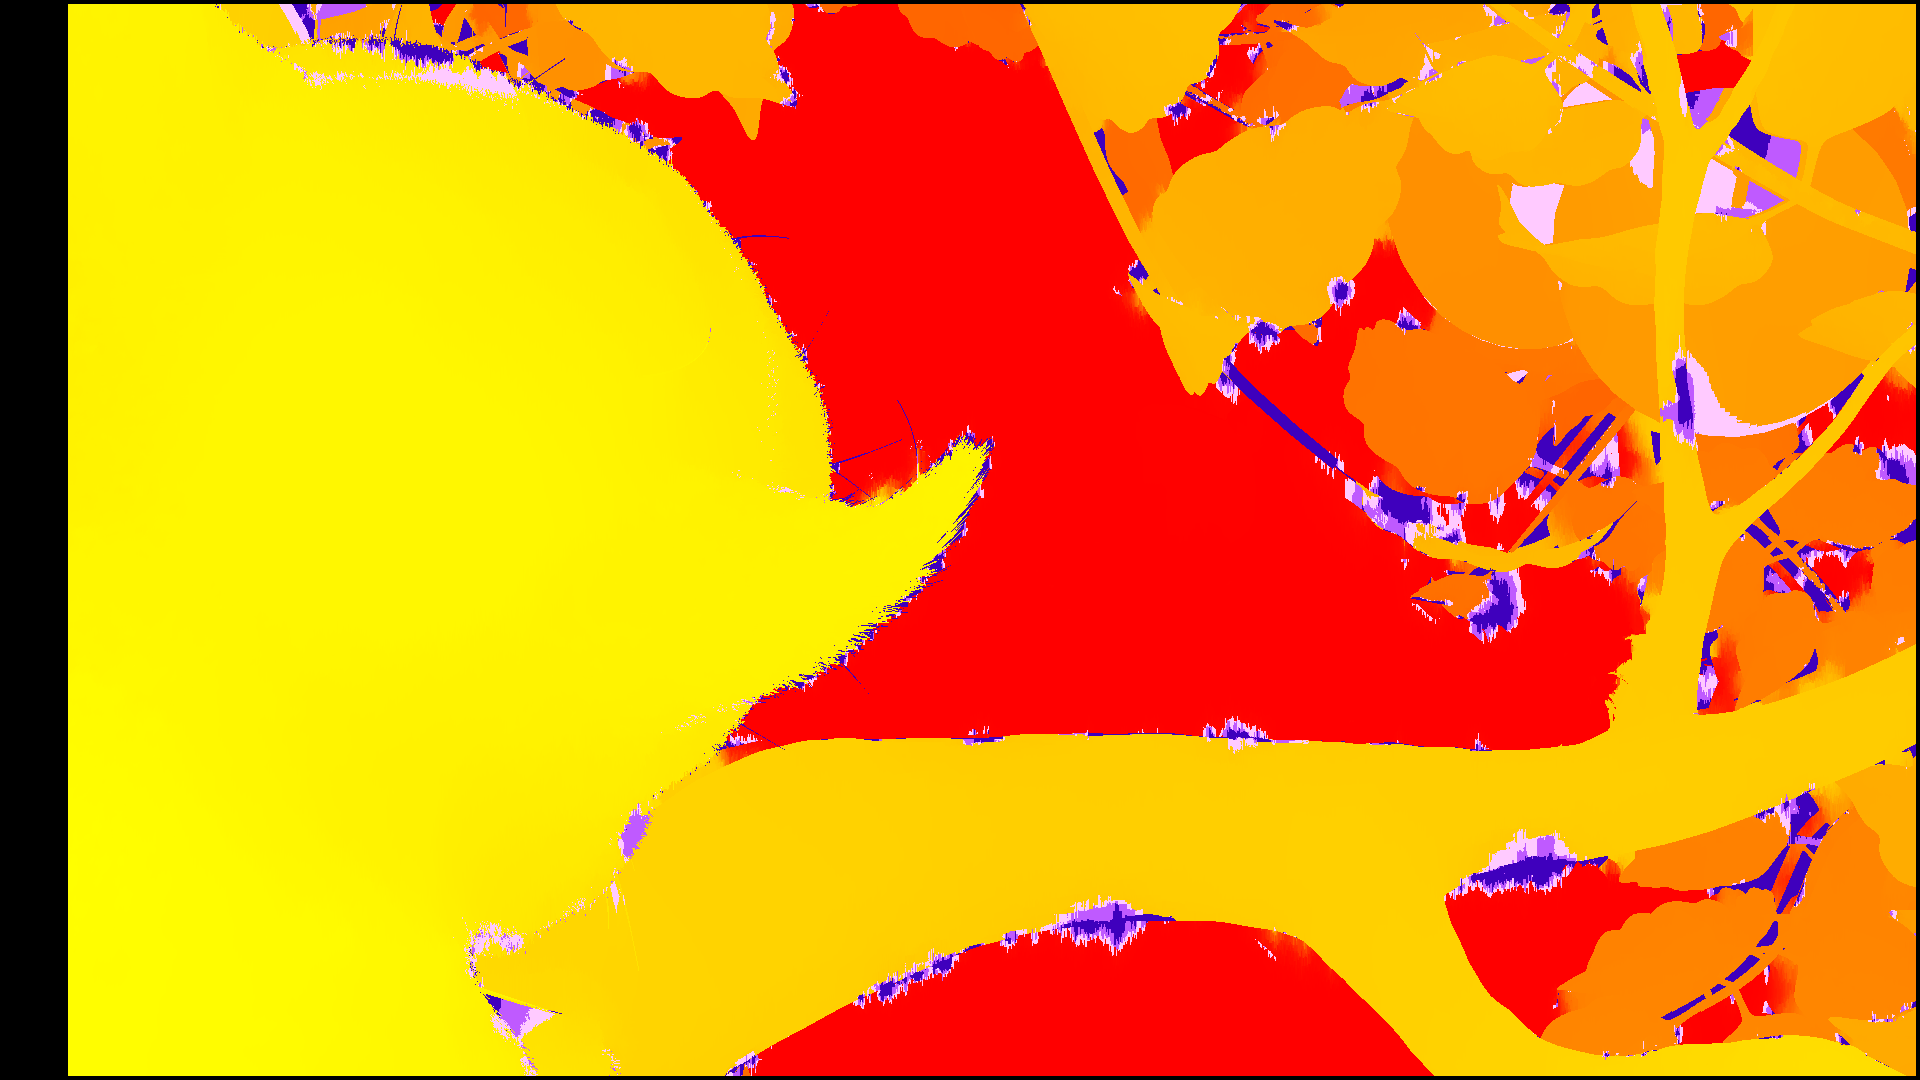
\includegraphics[width=0.48\textwidth]{../paper/src/images/evaluation/02-rabbit-elas.png}} &
  \end{tabular}
  \caption{Comparison of computed disparity maps regarding negative disparity.}
  \end{figure}
\end{frame}

\begin{frame}[fragile]{Results (8) - SVDDD performance}
  \begin{figure}
  \centering
  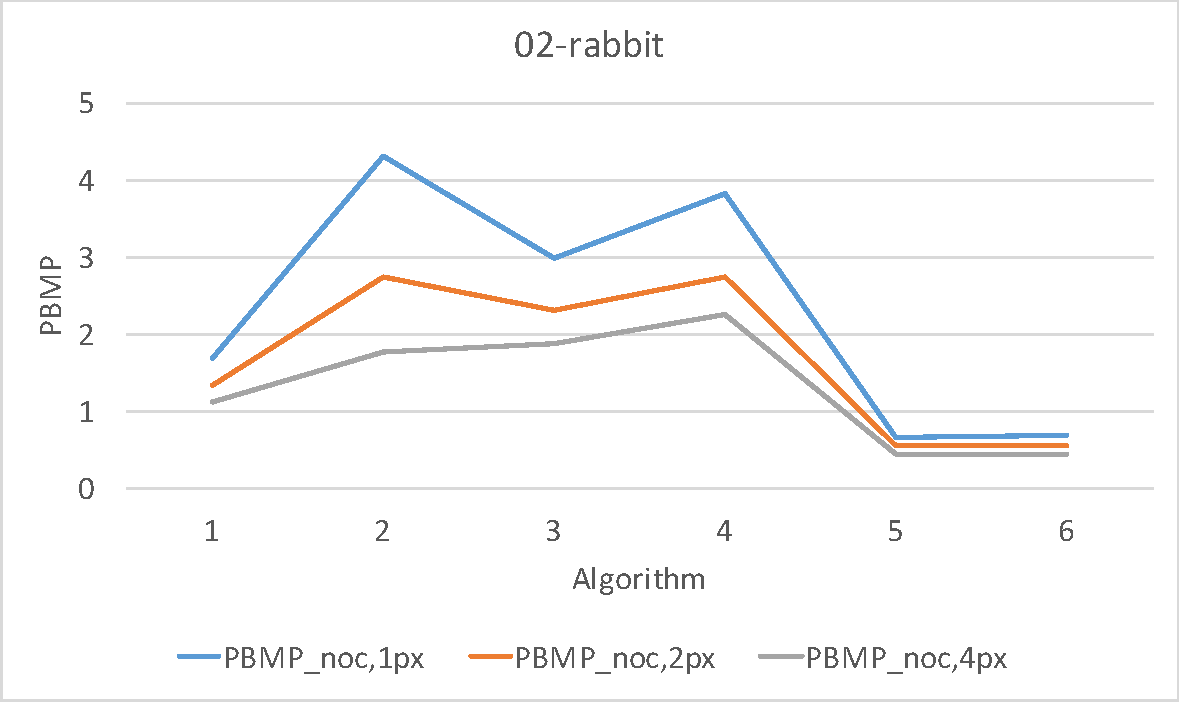
\includegraphics[width=0.9\textwidth]{../paper/src/images/evaluation/svddd/02-rabbit-plot.pdf}
  \caption[Performance of SVDDD rabbit scene]{Performance of SVDDD rabbit scene}
  \label{fig:eval-svddd-plot-rabbit}
  \end{figure}
\end{frame}

\begin{frame}[fragile]{Results (9) - SVDDD performance}
  \begin{table}
  \centering
  \scalebox{0.8}{
  \begin{tabular}{l|rrrrrr}
    & 1 CVSG & 2 CVBM & 3 ELAS & 4 MICM & 5 MGCE & 6 MGCS \\ \hline
  02-rabbit-neg & 58.62\% & \cellcolor{red!50}61.51\% & 59.99\% & 60.58\% & \cellcolor{green!50}57.12\% & 57.13\% \\
  02-rabbit & 1.68\% & \cellcolor{red!50}4.31\% & 2.98\% & 3.82\% & \cellcolor{green!50}0.65\% & 0.68\% \\
  03-apple & 1.69\% & \cellcolor{red!50}4.10\% & 3.11\% & 3.44\% & \cellcolor{green!50}0.63\% & 0.65\% \\ \hline
  $\varnothing$ (w/o neg) & 1.69\% & \cellcolor{red!50}4.21\% & 3.05\% & 3.63\% & \cellcolor{green!50}0.64\% & 0.67\%
  \end{tabular}
  }
  \caption{Result table for general performance of SVDDD (PBMP$_{noc,1px}$)}
  \end{table}
\end{frame}

\section{Conclusion and outlook}

\begin{frame}[fragile]{Conclusion}
  \begin{itemize}
    \item Surprise candidate ELAS
    \item Camera noise model
    \item SVDDD dataset
    \item Salient mask varies a bit
    \item Immense runtime differences
    \item Possible outliers in a scene
  \end{itemize}
\end{frame}

\begin{frame}[fragile]{Contributions}
  \begin{itemize}
    \item Generic disparity interface
    \item Evaluation Engine
    \item Mask creator
    \item Image diminisher
    \item Web result viewer
    \item Benchmark results
    \item Skeleton for stereo matcher
    \item Spatiotemporal stereo matcher
  \end{itemize}
\end{frame}

\begin{frame}[fragile]{Outlook}
  \begin{itemize}
    \item Motion saliency
    \item Enhancement of spatiotemporal matcher
    \item Holistic evaluation suite for modern disparity algorithm comparison
    \item Multi-view datasets
    \item High-resolution datasets
    \item Optical flow regarding spatiotemporal consistency
    \item Humans depth experience with neuronal networks
  \end{itemize}
\end{frame}

\plain{Questions?}

\end{document}
